\section{Laboratory work implementation}

\subsection{Tasks and Points}

În lucrarea de laborator dată au fost realizate următoarele sarcini:
\begin{enumerate}
\item au fost create 4 pagini statice:
	\begin{itemize}
	\item pagina principala;
	\item pagina de logare;
	\item pagina de înregistrare;
	\item pagina de delogare;
	\end{itemize}
\item a fost utilizată baza de date authentication pentru stocarea datelor despre utilizatori;
\item a fost utilizat Ajax-ul pentru configurarea și prelucrarea datelor;
\item a fost utilizat JSON-ul pentru datele primite în JavaScript de la altă aplicație;
\end{enumerate}


\subsection{Analiza lucrarii de laborator}

https://github.com/MarinaJechiuTI154/MIDPS

	În această lucrare de laborator a fost creat un site numit „Servicii foto”, constituit din 5 pagini statice, și anume:
	\begin{itemize}
	\item pagina principala;
	\item pagina de logare;
	\item pagina de înregistrare;
	\item pagina de delogare;
	\end{itemize}
	Pentru crearea paginilor a fost utilizat limbajul HTML. Pentru stilizare a fost implementate funcții ale limbajului CSS și JavaScript. Pentru efecte mai interesante s-a utilizat plugin-ul Stellar.js pentru mai multe efecte ale elementelor scroll. Pentru simplificarea lucrului cu animațiile și evenimentele a fost utilizată biblioteca jQwery.
	Legătura cu baza de date a fost asigurată cu ajutorul limbajului PHP. Au fost create pagini statice pentru logare și înregistrare, iar datele au fost stocate în baza de date authentication, tabelul users, alcătuit din 4 câmpuri:
	\begin{itemize}
	\item \textit{id} - atribuit automat în baza de date, autoindexându-se, fiindă asigurată unicitatea;
	\item \textit{username} - ales de utilizator și stocat conform alșegerii acestuia. Nu a fost asigurată unicitatea username-ului;
	\item textit{email} - ales de utilizator și stocat conform alșegerii acestuia. Nu a fost asigurată unicitatea email-ului;
	\item textit{password} - ales de utilizator și stocat conform alșegerii acestuia. Nu a fost asigurată unicitatea sau anumite condiții de securitate a parolei;
	\end{itemize}

	În momentul logării se face legătura cu baza de date și se verifică dacă există înregistrare cu asemenea username și password. Dacă există asemenea utilizator, acesta este automat redirecționat spre o nouă pagină principală: my-profil.php. În caz contrar, trebuie reintroduse datele de acces.
	Pentru interschimbarea datelor între paginile statice și JavaScript a fost folosite avantajele JSON (JavaScript Object Notation). Setul de tehnologii Ajax a fost implementat pentru a efectua o cerere la server. 
	
\subsection{Imagini}
% Exemplu de figura cu titlu, si referinta, label

\begin{figure}[!ht]
\centering
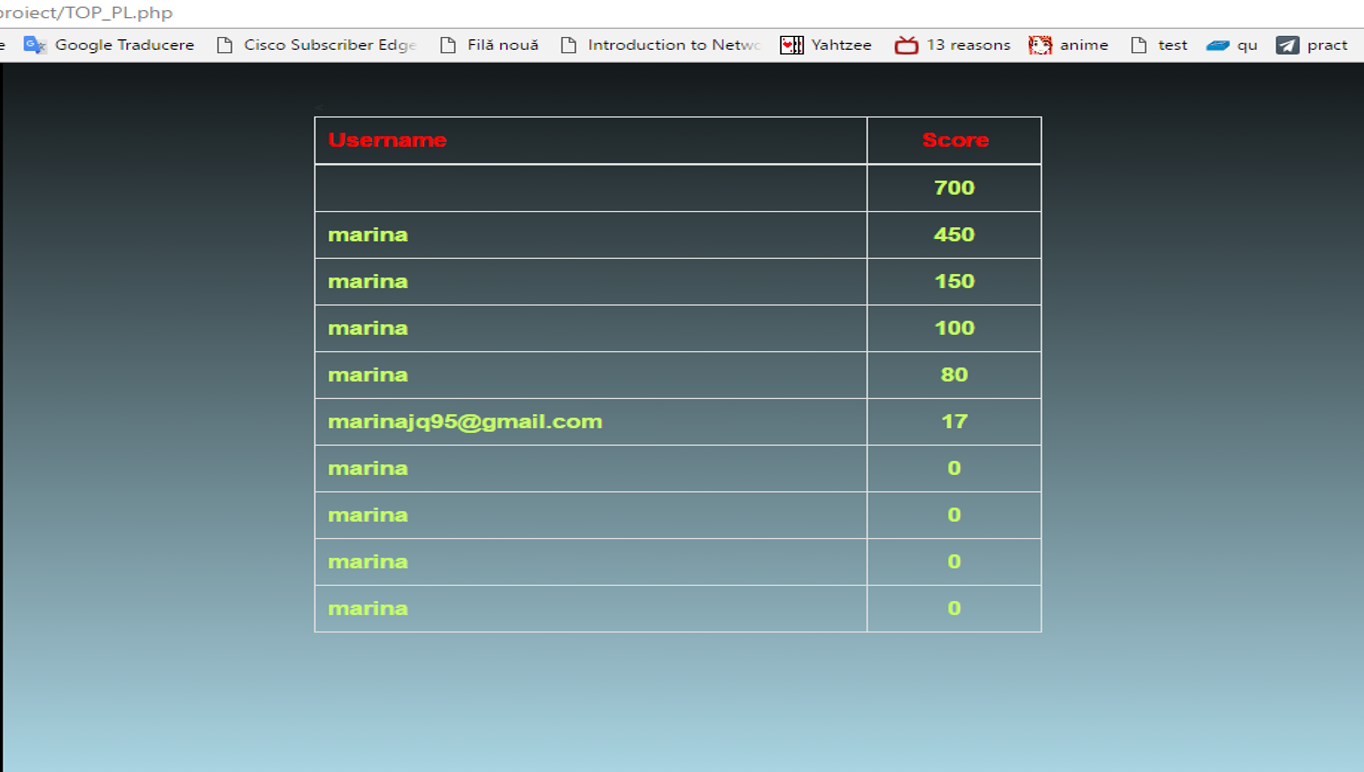
\includegraphics[width=1.0\textwidth]{1}
\caption{Pagina principală}

\end{figure}


\begin{figure}[!ht]
\centering

\includegraphics[width=1.0\textwidth]{2}
\caption{Pagina de înregistrare}

\end{figure}

\begin{figure}[!ht]
\centering
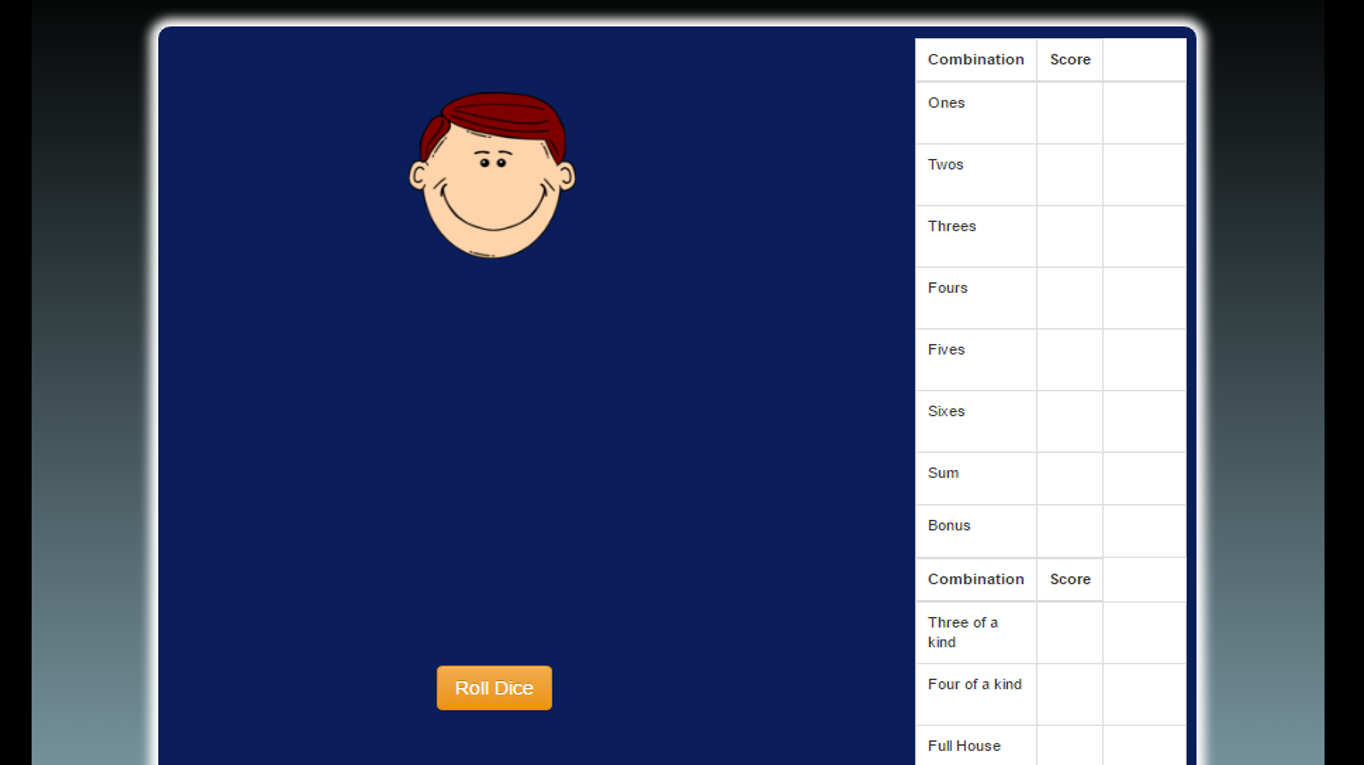
\includegraphics[width=1.0\textwidth]{3}
\caption{Pagina de logare}

\end{figure}

\begin{figure}[!ht]
\centering
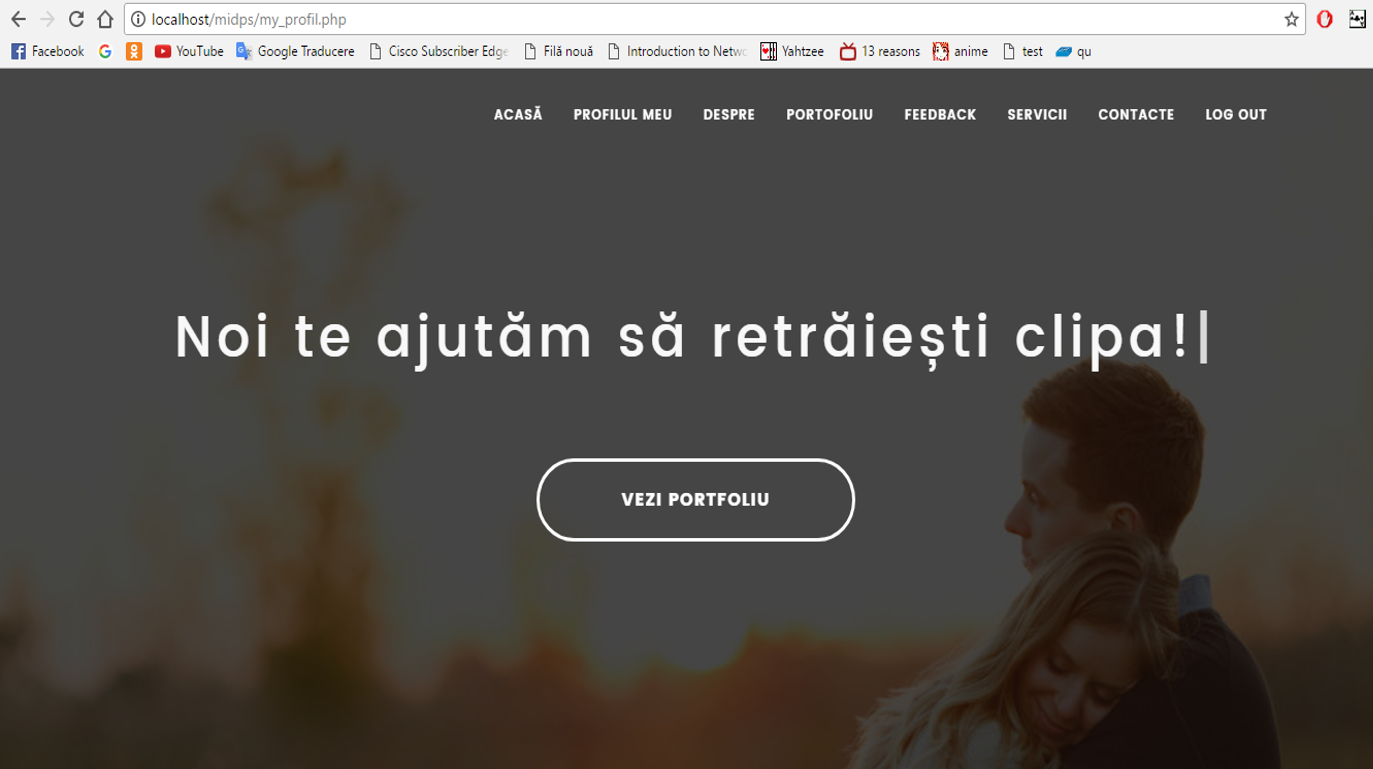
\includegraphics[width=1.0\textwidth]{4}
\caption{Pagina principală după logare}

\end{figure}

\begin{figure}[!ht]
\centering

\includegraphics[width=1.0\textwidth]{5}
\caption{Portofoliu}

\end{figure}

\begin{figure}[!ht]
\centering
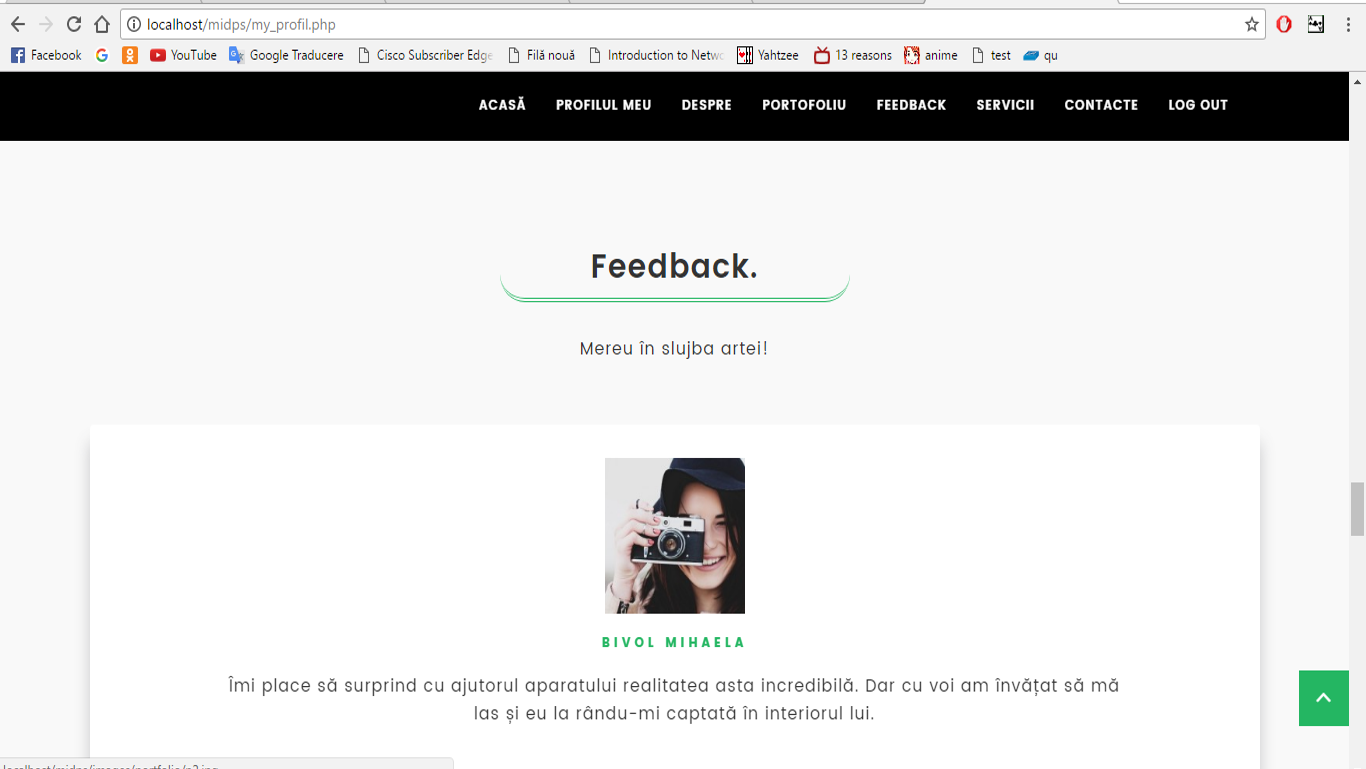
\includegraphics[width=1.0\textwidth]{6}
\caption{Feed back}

\end{figure}

\begin{figure}[!ht]
\centering
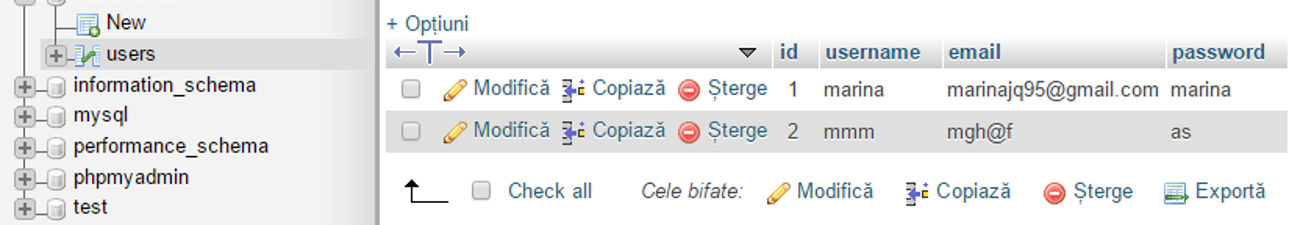
\includegraphics[width=1.0\textwidth]{7}
\caption{Baza de date }}

\end{figure}
% Exemplu de listing. Cum sa adaugi cod sursa in functie de limbajul de programare



% Exemplu de tabel. El poate fi efectuat si exportat in forma online: 
% http://www.tablesgenerator.com/






\clearpage